\section{Grader} \label{sec:grader}
Når man regner på grafer, som vi vil gøre senere i projektet, kan det være brugbart at have styr på, hvor mange kanter der er incidente med en knude. Dertil bruger man følgende definition:

\begin{defn}[Grader] \label{defn:grader}
I en ikke-orienteret graf, $G = (V,E)$ er en knude, $v$'s antal \emph{grader}, $\deg(v)$, det antal kanter, $E$, som er incidente med $v$. Dermed skal det gælde, at
\begin{equation}
\deg(v)=\sum_{i=0} ^{n} \{u,v\}|u,v \in V .
\end{equation}
\end{defn}

En løkke bidrager to gange til knudens grad, da kanten både starter og stopper i denne knude.

\begin{exmp} \label{ex:grader}

Graderne på \autoref{fig:grader} er $\deg(v_{1})=3, \ \deg(v_{2})=3, \ \deg(v_{3})=4$ og $\deg(v_{4})=4$. En knudes grader afgøres altså af, hvor mange naboer knuden har, medmindre knuden har en løkke, da man her kun siger, at den er nabo med sig selv én gang, men det tæller dobbelt i antallet af grader.


\begin{figure}[H]
\centering
	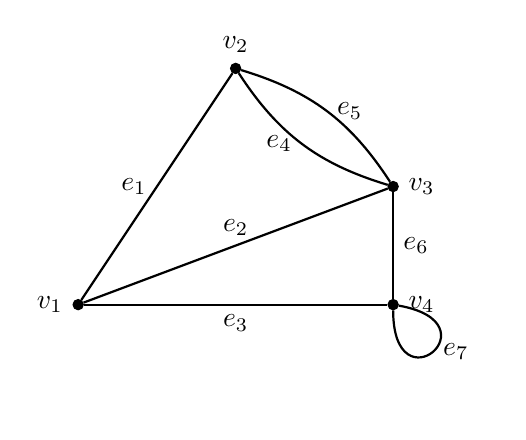
\begin{tikzpicture}[every loop/.style={}]
      \tikzset{enclosed/.style={draw, circle, inner sep=0pt, minimum size=.13cm, fill=black}}
%% Vertices
      	\node[enclosed, label={left: $v_1$}] (v1) at (0,0) {};
      	\node[enclosed, label={above: $v_2$}] (v2) at (2,3) {};
    	\node[enclosed, label={right: $v_3$}] (v3) at (4,1.5) {};
  	    \node[enclosed, label={right: $v_4$}] (v4) at (4,0) {};
%Edges
		\path[thick] (v2) edge [bend right=20] node[midway, left] {$e_4$} (v3);
		\path[thick] (v3) edge [bend right=20] node[midway, right] {$e_5$} (v2);
		\path[thick] (v1) edge node[midway, above] {$e_2$} (v3);
		\path[thick] (v1) edge node[midway, below] {$e_3$} (v4);
		\path[thick] (v1) edge node[midway, left] {$e_1$} (v2);
		\path[thick] (v3) edge node[midway, right] {$e_6$} (v4);
		\path[thick] (v4) edge [out=270,in=350,looseness=35] node[right] {$e_7$} (v4);
	\end{tikzpicture}
	\caption{Pseudograf.}
	\label{fig:grader}
\end{figure}


\end{exmp}

\begin{thm}
Lad grafen, $G = (V,E)$ være en ikke-orienteret graf med E antal kanter. Punktet $v$ har $deg(v)$ antal grader, gør det sig gældende, at
\begin{equation}
2 \cdot |E|= \sum_{v \in V} { } \deg(v).
\end{equation}
Dette gælder, så længe grafen ikke er uendelig.
\end{thm}
Hvis vi har en ikke-orienteret, endelig graf, kan man altså finde antallet af kanter i grafen ved at lægge summen af hvert punkts grader sammen og dividere dette tal med to.
Det vil sige, at for ikke-orienterede grafer kan man finde antallet af kanter ved at lægge summen af graderne for hvert hjørne sammen, og derefter dividere det med to. Dette vil blive illustreret i eksempel 2.2.7.

\begin{proof}
Som det fremgår af Definition \ref{def:graf}, er kanter, $E \subseteq \{\{u,v\}|u,v \in V \}$. Hver kant i grafen er altså incident med to punkter, eller med det samme punkt to gange, hvis der er tale om en løkke. Hvis en kant er incident med en knude, bidrager denne kant til knudens grader, $\deg{v}$. Hver kant bidrager altså to gange til det samlede antal grader. Derfor vil hele grafens antal grader, $\sum_{v \in V} { } \deg(v)$, være dobbelt så stor, som antallet af kanter i denne graf, $|E|$. Derfor får vi at 
\begin{equation}
2 \cdot |E|= \sum_{v \in V} { } \deg(v).
\end{equation} 
\end{proof}
